%
\documentclass[journal]{IEEEtran}
%


% *** CITATION PACKAGES ***
%
%\usepackage{cite}
% cite.sty was written by Donald Arseneau
% V1.6 and later of IEEEtran pre-defines the format of the cite.sty package
% \cite{} output to follow that of IEEE. Loading the cite package will
% result in citation numbers being automatically sorted and properly
% "compressed/ranged". e.g., [1], [9], [2], [7], [5], [6] without using
% cite.sty will become [1], [2], [5]--[7], [9] using cite.sty. cite.sty's
% \cite will automatically add leading space, if needed. Use cite.sty's
% noadjust option (cite.sty V3.8 and later) if you want to turn this off.
% cite.sty is already installed on most LaTeX systems. Be sure and use
% version 4.0 (2003-05-27) and later if using hyperref.sty. cite.sty does
% not currently provide for hyperlinked citations.
% The latest version can be obtained at:
% http://www.ctan.org/tex-archive/macros/latex/contrib/cite/
% The documentation is contained in the cite.sty file itself.


%\usepackage[numbered,framed]{matlab-prettifier}
%\usepackage{color}
\usepackage[usenames,dvipsnames,svgnames,table]{xcolor}
\usepackage{listings}



% *** GRAPHICS RELATED PACKAGES ***
\usepackage{ifpdf}
%\usepackage{paralist}
\usepackage{amsfonts}
% \usepackage{subfig}
\usepackage{subcaption}
  \usepackage{epstopdf}
   \ifpdf
	\usepackage{graphicx}
  	\graphicspath{{Pics/}}  
  	\DeclareGraphicsExtensions{.pdf,.jep,.png}
 \else
  \usepackage[dvips]{graphicx}
  \graphicspath{images/}
  \DeclareGraphicsExtensions{.eps}
 \fi
 
\usepackage{hyperref}
\def\figureautorefname{Fig.}


%
\ifCLASSINFOpdf
  % \usepackage[pdftex]{graphicx}
  % declare the path(s) where your graphic files are
  % \graphicspath{{../pdf/}{../jpeg/}}
  % and their extensions so you won't have to specify these with
  % every instance of \includegraphics
  % \DeclareGraphicsExtensions{.pdf,.jpeg,.png}
\else
  % or other class option (dvipsone, dvipdf, if not using dvips). graphicx
  % will default to the driver specified in the system graphics.cfg if no
  % driver is specified.
  % \usepackage[dvips]{graphicx}
  % declare the path(s) where your graphic files are
  % \graphicspath{{../eps/}}
  % and their extensions so you won't have to specify these with
  % every instance of \includegraphics
  % \DeclareGraphicsExtensions{.eps}
\fi
% graphicx was written by David Carlisle and Sebastian Rahtz. It is
% required if you want graphics, photos, etc. graphicx.sty is already
% installed on most LaTeX systems. The latest version and documentation can
% be obtained at: 
% http://www.ctan.org/tex-archive/macros/latex/required/graphics/
% Another good source of documentation is "Using Imported Graphics in
% LaTeX2e" by Keith Reckdahl which can be found as epslatex.ps or
% epslatex.pdf at: http://www.ctan.org/tex-archive/info/
%
% latex, and pdflatex in dvi mode, support graphics in encapsulated
% postscript (.eps) format. pdflatex in pdf mode supports graphics
% in .pdf, .jpeg, .png and .mps (metapost) formats. Users should ensure
% that all non-photo figures use a vector format (.eps, .pdf, .mps) and
% not a bitmapped formats (.jpeg, .png). IEEE frowns on bitmapped formats
% which can result in "jaggedy"/blurry rendering of lines and letters as
% well as large increases in file sizes.
%
% You can find documentation about the pdfTeX application at:
% http://www.tug.org/applications/pdftex





% *** MATH PACKAGES ***
%
\usepackage[cmex10]{amsmath}
% A popular package from the American Mathematical Society that provides
% many useful and powerful commands for dealing with mathematics. If using
% it, be sure to load this package with the cmex10 option to ensure that
% only type 1 fonts will utilized at all point sizes. Without this option,
% it is possible that some math symbols, particularly those within
% footnotes, will be rendered in bitmap form which will result in a
% document that can not be IEEE Xplore compliant!
%
% Also, note that the amsmath package sets \interdisplaylinepenalty to 10000
% thus preventing page breaks from occurring within multiline equations. Use:
%\interdisplaylinepenalty=2500
% after loading amsmath to restore such page breaks as IEEEtran.cls normally
% does. amsmath.sty is already installed on most LaTeX systems. The latest
% version and documentation can be obtained at:
% http://www.ctan.org/tex-archive/macros/latex/required/amslatex/math/





% *** SPECIALIZED LIST PACKAGES ***
%
\usepackage{algorithmic}
% algorithmic.sty was written by Peter Williams and Rogerio Brito.
% This package provides an algorithmic environment fo describing algorithms.
% You can use the algorithmic environment in-text or within a figure
% environment to provide for a floating algorithm. Do NOT use the algorithm
% floating environment provided by algorithm.sty (by the same authors) or
% algorithm2e.sty (by Christophe Fiorio) as IEEE does not use dedicated
% algorithm float types and packages that provide these will not provide
% correct IEEE style captions. The latest version and documentation of
% algorithmic.sty can be obtained at:
% http://www.ctan.org/tex-archive/macros/latex/contrib/algorithms/
% There is also a support site at:
% http://algorithms.berlios.de/index.html
% Also of interest may be the (relatively newer and more customizable)
% algorithmicx.sty package by Szasz Janos:
% http://www.ctan.org/tex-archive/macros/latex/contrib/algorithmicx/




% *** ALIGNMENT PACKAGES ***
%
\usepackage{array}
% Frank Mittelbach's and David Carlisle's array.sty patches and improves
% the standard LaTeX2e array and tabular environments to provide better
% appearance and additional user controls. As the default LaTeX2e table
% generation code is lacking to the point of almost being broken with
% respect to the quality of the end results, all users are strongly
% advised to use an enhanced (at the very least that provided by array.sty)
% set of table tools. array.sty is already installed on most systems. The
% latest version and documentation can be obtained at:
% http://www.ctan.org/tex-archive/macros/latex/required/tools/

% *** PDF, URL AND HYPERLINK PACKAGES ***
%
\usepackage{url}

% correct bad hyphenation here
\hyphenation{op-tical net-works semi-conduc-tor}

\usepackage{hyperref}

\begin{document}

%
% paper title
% can use linebreaks \\ within to get better formatting as desired
\title{Title}
%

\author{Roni Hyt\"{o}nen,~\IEEEmembership{r.h.hytonen@student.utwente.nl,~s1887033,~BME}  
      
        and~Dani\"el Cox,~\IEEEmembership{d.w.s.cox@student.utwente.nl,~s1228579,~APH}% <-this % stops a space

% <-this % stops a space
}



% The paper headers
\markboth{\today, Image processing and Computer Vision}%
{Project 3: 3D face reconstruction}
% The only time the second header will appear is for the odd numbered pages
% after the title page when using the twoside option.


% make the title area
\maketitle


\begin{abstract}
%\boldmath
In this project three stereoscopic photographs are combined to form a three-dimensional face reconstruction. 
For this purpose the camera parameters are defined, stereo images rectified, and a disparity map is computed.
Additionally, a background removal is implemented, as well as a relaxation method for interpolation of regions where reconstruction failed.

\textit{Add a short abstract here containing at most 100 words. Abstracts do not contain symbols, special characters, math, or references. Describe the context shortly, and summarize the research question and the main items from the discussion.}
\end{abstract}
% IEEEtran.cls defaults to using nonbold math in the Abstract.
% This preserves the distinction between vectors and scalars. However,
% if the journal you are submitting to favors bold math in the abstract,
% then you can use LaTeX's standard command \boldmath at the very start
% of the abstract to achieve this. Many IEEE journals frown on math
% in the abstract anyway.

% Note that keywords are not normally used for peerreview papers.
\begin{IEEEkeywords}
four key words in alphabetical order, separated by commas.
\end{IEEEkeywords}


\IEEEpeerreviewmaketitle



\section{Introduction}
% The very first letter is a 2 line initial drop letter followed
% by the rest of the first word in caps.
% 
% form to use if the first word consists of a single letter:
% \IEEEPARstart{A}{demo} file is ....
% 
% form to use if you need the single drop letter followed by
% normal text (unknown if ever used by IEEE):
% \IEEEPARstart{A}{}demo file is ....
% 
% Some journals put the first two words in caps:
% \IEEEPARstart{T}{his demo} file is ....
% 
% Here we have the typical use of a "T" for an initial drop letter
% and "HIS" in caps to complete the first word.
\IEEEPARstart{3}{D} face reconstruction is a relevant problem for e.g. the purposes of face recognition and animation \cite{3D_Peng}.
The most novel methods include complex modalities such as laser scanning and multi-view cinematography, but the same task can be completed with a pair of stereo images \cite{Creation_Krutikova}.

In this project three images of subject's bust are used to first reconstruct two depth images, that are then combined to comprise a full frontal 3D image.
For this stereo calibrations of the cameras and image rectifications are performed, the disparity map is computed, and the background is removed.
From the disparity maps depth images are reconstructed, and those are then converted to surface meshes, which are finally combined to yield the 3D mesh of the full bust.


introduction contains (1) a background, (2) the definition of the problem that is addressed possibly with a research question and subquestions, (3) a short outline of the report.

Note 1: the problem is \textbf{not} how to create a Matlab function. The definition of the problem should be at a much higher level of abstraction.

Note 2: The introduction should be readable for a less technically skilled audience, e.g. a clinician, or a manager. Therefore, the introduction does not contain symbols, special characters, or math. 

% You must have at least 2 lines in the paragraph with the drop letter
% (should never be an issue)
\section{Methods and Materials}

\subsection{Materials}
A set of twenty calibration images was used to perform the stereo camera calibration. 
The images were taken simultaneously from three sides with a calibration checkerboard (10mm squares) in view.
Accordingly, the subjects consisted of three persons, imaged with the three-camera system so, that one image was taken straight from the middle, one from the left and one from the right. 
In total five images of each subject were taken, each with a different facial expression.


\subsection{Methods}
\subsubsection{Analysis}
Start with defining the overview of the problem in a more mathematical context. What is the input? What is the desired output? (Introduce mathematical symbols for the input and output variables). What is in rough steps the strategy to get the output from the input?
 
Next, define the subtasks in more detail. For each subtask, introduce variables whenever needed, and set-up the mathematical relations (equations) between these variables, possibly combined with pseudo code.  Do \textbf{no}t use Matlab code. Describe your algorithm such that the principle of operation becomes clear. For that, use �mathematical style� pseudo code. See: \href{https://en.wikipedia.org/wiki/Pseudocode\#https://en.wikipedia.org/wiki/Pseudocode}{https://en.wikipedia.org/wiki/Pseudocode} and pseudo-code examples provided in \href{https://en.wikipedia.org/wiki/Category:Articles_with_example_pseudocode\#https://en.wikipedia.org/wiki/Category:Articles_with_example_pseudocode}{https://en.wikipedia.org/wiki/Category:Articles\_with\_example \_pseudocode}. The only place in the report that contains Matlab code is the appendix (you should add your listing as an annex).

\subsubsection{Background Detection}
A large part of the images consists uniformly coloured background.
Because the tone of the background is very similar to skin colour, colour-based segmentation methods yield easily incorrect results. 
However, since the background is fairly smooth, whereas the foreground with person is more heavily textured. 
Because of this an edge-based segmentation is a logical choice for background removal.

The method itself has been implemented in four simple steps, also illustrated in \autoref{fig:backgroundRemoval}.
First, the colour image is converted to gray scale in order to facilitate subsequent steps.
Then the intensity gradients in the image are detected using Canny method.
Because of the nature of bust images, there are very few edges arising from the background, and numerous ones from the bust itself.
However, there are multiple breaks in the bust outline, as the skin tone and intensity matches that of the background. 
Thus a morphological closing is required in order to connect the outline of the bust before finally morphologically filling the image.


\begin{figure}
\centering
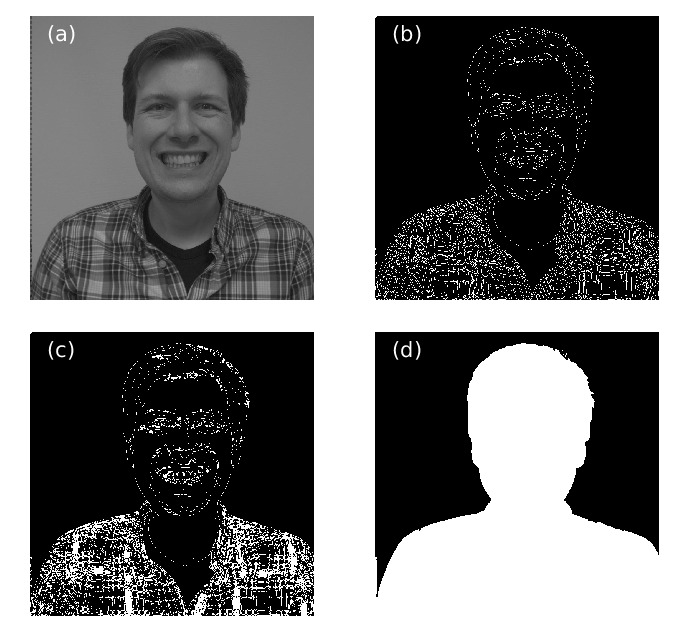
\includegraphics[width=\linewidth]{BGRemoval.png}
\caption{Steps of background detection algorithm:\\
\textbf{(a)} The gray scale bust image\\
\textbf{(b)} Edge detection\\
\textbf{(c)} Morphological closing\\
\textbf{(d)} Hole filling
}
\label{fig:backgroundRemoval}
\end{figure}


\subsubsection{Image normalisation}

The bust stereo images have slightly different lighting effects for each angle, which may cause instability later on.
For this purpose both left and right stereo images were normalized to correspond the middle one in regards to the mean and variance of their intensities.

The variance and mean were normalised as 

\begin{align}
J_{x} &= I_{x} \times \dfrac{\texttt{var}(I_{mid})}{\texttt{var}(I_x)}\\
K_{x} &= J_{x} \times \dfrac{\texttt{mean}(I_{mid})}{\texttt{mean}(J_x)},
\end{align}

\noindent where I, J and K are the non-normalised, variance normalised, mean normalised images, respectively.


\subsubsection{Stereo calibration}

The three-camera system was calibrated using the calibration image set explained in the section \textit{Materials}. 
The calibration was done in pairs, pairing up the middle image with both left and right images.
A three-coefficient stereo calibration was performed using Matlab's \textit{Stereo Camera Calibrator}.


\subsubsection{Rectification}

The image pairs were rectified (i.e. projected onto a common image plane) by using Matlab's \textit{rectifyStereoImages}-function with the determined stereo calibration parameters.
The rectified images have each row of pixels corresponding each other, making the calculation of disparity simpler.


\subsubsection{Disparity}

For the rectified images each world point lies on the same row, but at the different column. 
The distance between the two columns, or the disparity, was computed using Matlab's \textit{disparity}-function with block size of 5 and disparity range of 0 and 640. %%% refer to disparity function in appendix?

The disparity was computed separately for each colour channel. If the disparity for a certain pixel is unresolved, it returns a 0. The final disparity value for each pixel was calculated as the mean of successfully determined values. Though this method slightly increases the number of matched pixels, this does mean there will still be `gaps' in the disparity map for all the parts that are fully unresolved. These can be observed in figure \ref{fig:disparity-rgb}. In the next step, these gaps are filled with sensible values using an interpolation algorithm.

\begin{figure}[h]
    \centering
    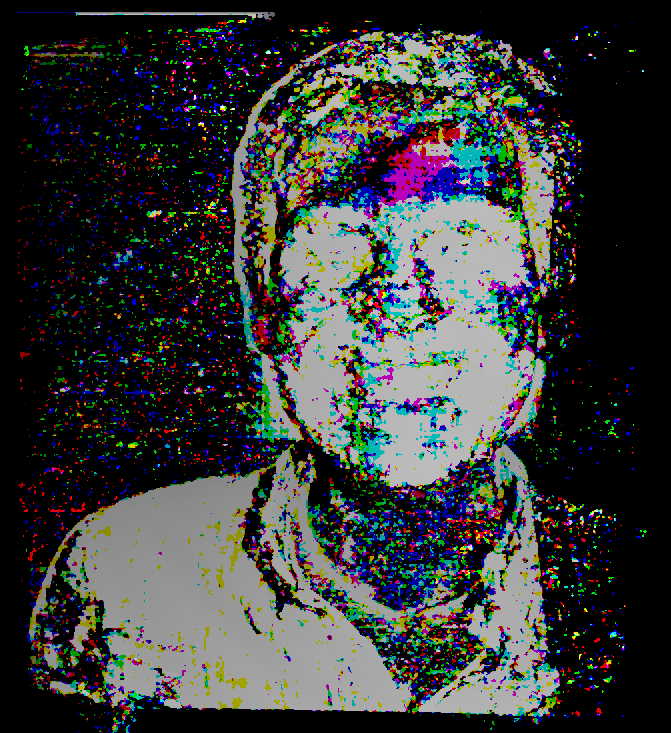
\includegraphics[width=0.6\linewidth]{Pics/disparity-RGB.png}
    \caption{Disparity map for the RGB channels. For the colored pixels, only one or two channels have a disparity match. For the grey or white pixels, all channels are resolved. Black represents fully unresolved pixels.}
    \label{fig:disparity-rgb}
\end{figure}

% If only one colour channel yields a result and the two others fail, the result is discarded altogether and the disparity is acquired by means of interpolation. ----> This is no longer used, as it didn't seem to be an effective way of removing errors.


\subsubsection{Interpolation}
The interpolation algorithm fills in gaps of an input image using iterative relaxation. It computes sensible values for which the Laplacian is minimized, by setting each pixel to the average of the surrounding values. `Known' values will be used as boundary conditions. Furthermore, every iteration, a convergence value (squared sum of difference with previous iteration) is compared to a target value. The algorithm stops if either this target convergence value is reached or the number of iterations has reached its designated maximum value.

\begin{figure}[h]
    \centering
    \begin{subfigure}[t]{0.45\linewidth}
        \centering
        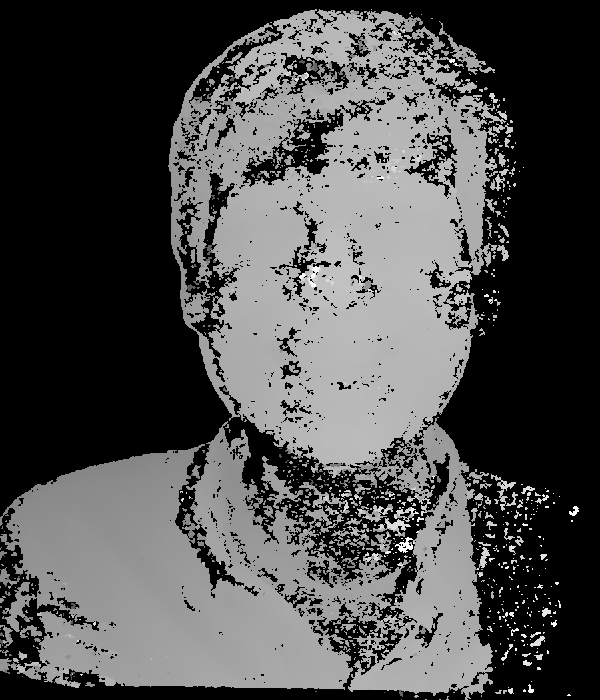
\includegraphics[width=\linewidth]{Pics/disparity-gaps.png}
        \caption{Disparity map contains gaps of unresolved values.}
        \label{fig:disparity-gaps}
    \end{subfigure}
    ~
    \begin{subfigure}[t]{0.45\linewidth}
        \centering
        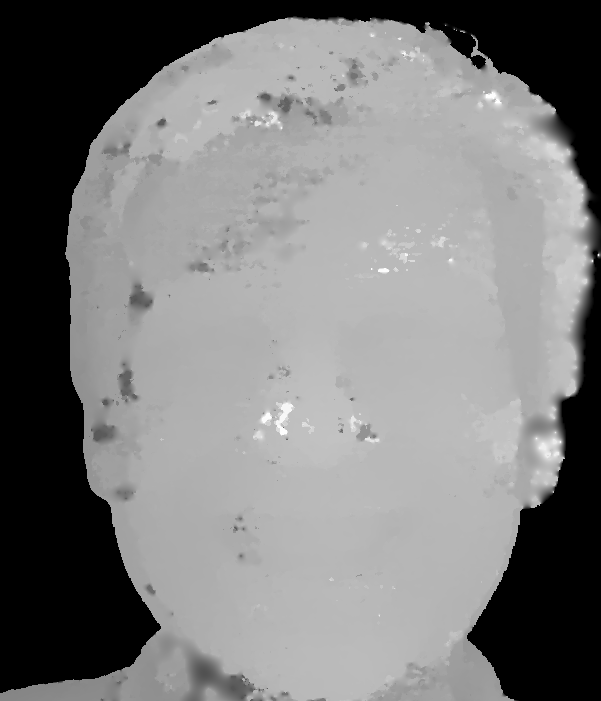
\includegraphics[width=\linewidth]{Pics/disparity-fill.png}
        \caption{Disparity gaps are filled using iterative relaxation.}
        \label{fig:disparity-fill}
    \end{subfigure}
    ~
    \begin{subfigure}[t]{0.45\linewidth}
        \centering
        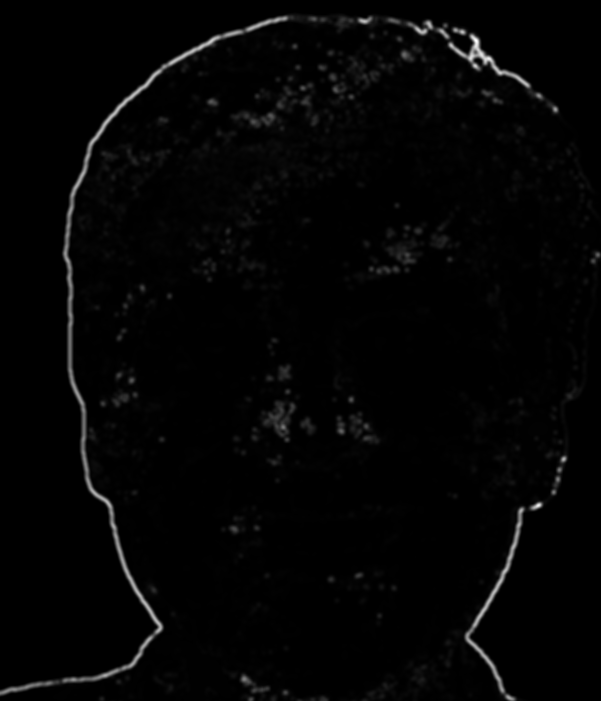
\includegraphics[width=\linewidth]{Pics/disparity-lapf.png}
        \caption{Disparity map contains errors which generally show up as `spiky' patches. Laplacian filter detects these patches.}
        \label{fig:disparity-lapf}
    \end{subfigure}
    ~
    \begin{subfigure}[t]{0.45\linewidth}
        \centering
        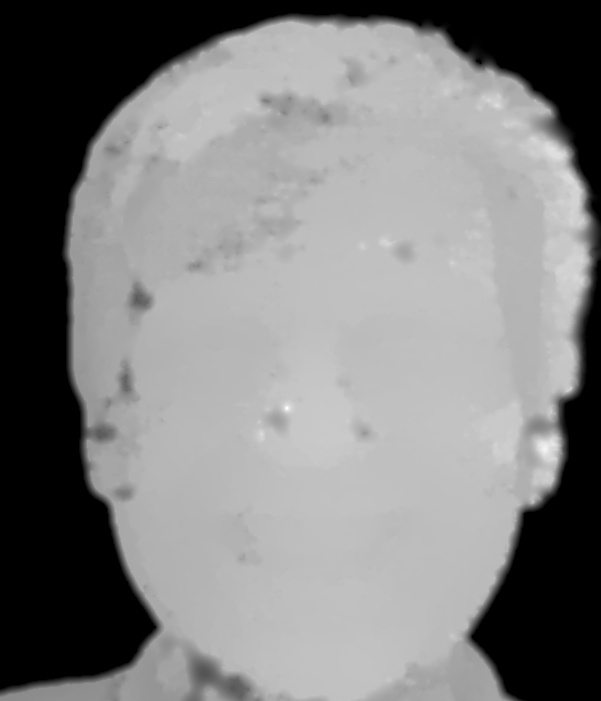
\includegraphics[width=\linewidth]{Pics/disparity-flf.png}
        \caption{By means of a threshold, the spiky areas are removed and filled with the relaxation function.}
        \label{fig:disparity-flf}
    \end{subfigure}
    \caption{Disparity gaps interpolation and filtering.}
    \label{fig:disparity-fillgap}
\end{figure}


\subsubsection{Performance evaluation}
For a performance evaluation, you often need to set-up an experiment. Describe the (protocol of the) experiment. Describe how the outcome of the experiment will be processed. Often, you need reference values, i.e. a gold standard, or a ground truth. Describe how this is achieved. If the processing is done statistically, mention the statistical test or statistical inference method.


\section{Results}

The results for reconstruction are presented in Figures \ref{fig:result_S1}--\ref{fig:result_S3}, and as can be seen, the depth of different features was mapped successfully for most parts.
Especially the areas with higher amounts of texture, such as hair, eyes, mouth and part of the shirt were reconstructed very well. 
Accordingly, the algorithm struggled in regions with only little texture, such as forehead and neck, as can be seen from figure \ref{fig:disparity-gaps}.


\begin{figure}
    \centering
    \begin{subfigure}[t]{\linewidth}
        \centering
        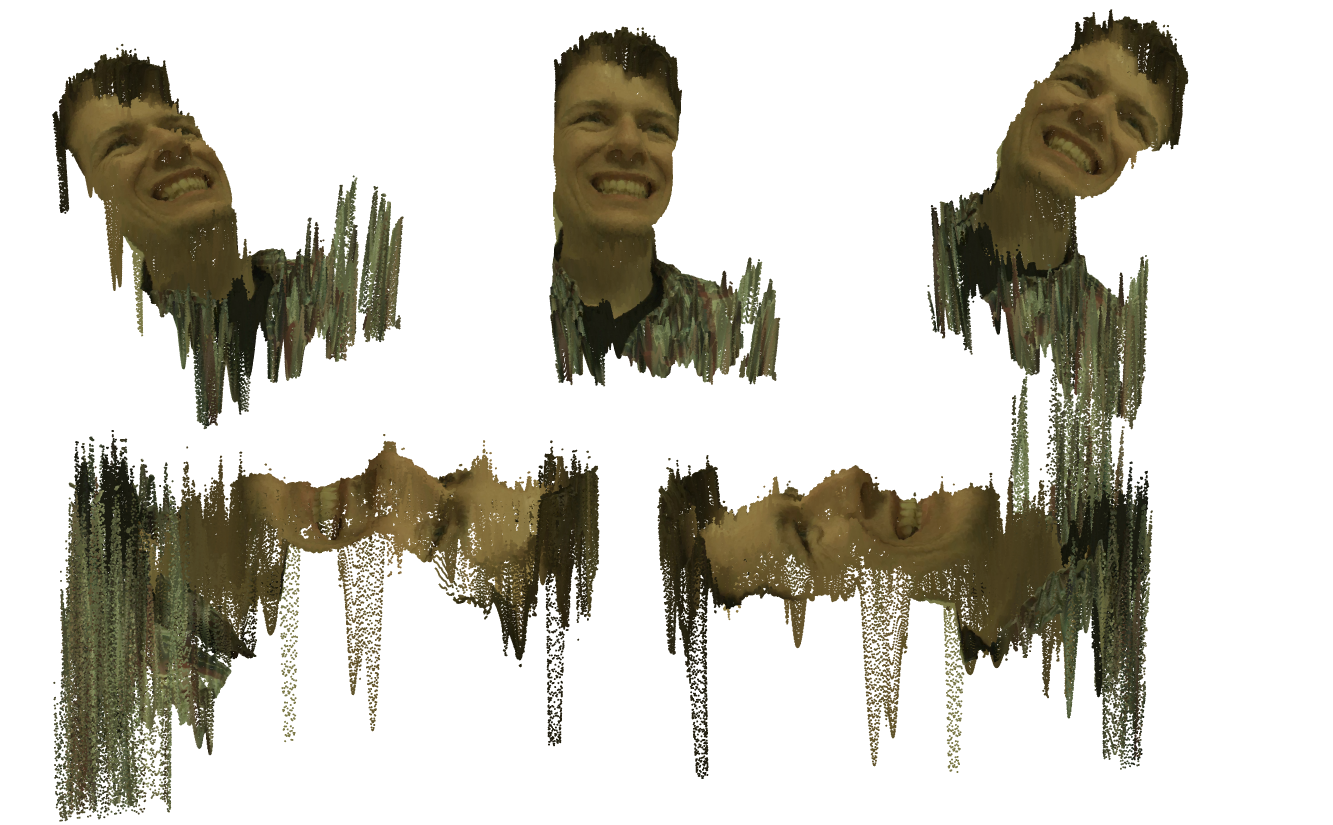
\includegraphics[width=\linewidth]{result_S1_R}
		\caption{}
		\label{fig:result_S1}
    \end{subfigure}
    
    \begin{subfigure}[t]{\linewidth}
        \centering
		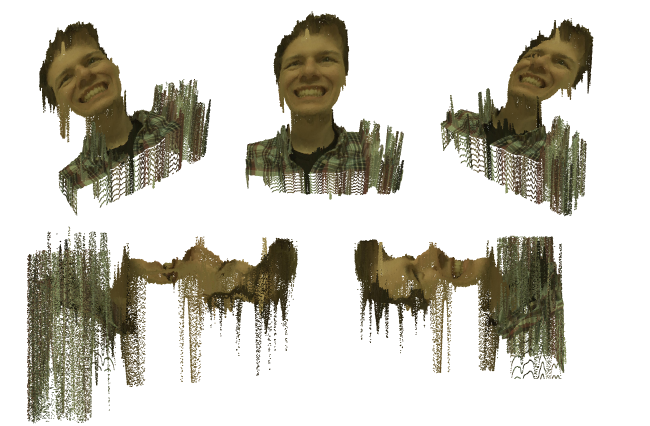
\includegraphics[width=\linewidth]{result_S1_L}
		\caption{}
		\label{fig:result_S2}
    \end{subfigure}
    
    \caption{Reconstruction results for subject 1 from left \textbf{(a)} and right \textbf{(b)} views.}
    \label{fig:results-reconstruction}

\end{figure}

The inter-subject variation of the results was considerable. The main factor was the amount of detail in the area: the subjects' hair, clothes, and the areas around mouth and eyes were properly reconstructed in virtually all subjects. 
On the contrary, the more there were featureless regions, such as smooth skin or solid colour clothing. This is especially visible in subject 3 in figure \ref{fig:result_S3}.

Here, you give the results of what is described in Section II: tables, images and/or graphs. The accompanying text of these tables, images and/or graphs clarifies how they are related to the methods described in Section II.
 
If you have any remarkable observations, mention and describe them here, but without an interpretation, explanation, or meaning.
Do not introduce new methods in this section. And do not give an interpretation or a judgement of these results.


\section{Discussion}

The results could be further improved by combining the left and right meshes to yield a more complete view of the face. 
However, in this case since the reconstruction of the left side was slanted and of very poor quality, this would've only made the outcome worse.
But had the outcome been different, the images could've been combined e.g. by means of iterative closest point matching, or by fitting both of them on top of a face archetype.

The most probable explanation for the poor performance on the left side images is that there was something wrong with the disparity computation...
It's also possible, that the problems were caused by the viewing angle, and  rectification of the disparity map before proceeding would've yielded better results.

Removal of the background from the image by masking proved to be an efficient approach. 
Alternatively, the unwanted background could be sought to be removed by discriminating on the basis of the disparity. 
The effect of image normalization was not studied.

The number of calibration images used was also found to affect the results.
While the main results were acquired using twenty calibration images per camera, the result by using only ten is presented Appendix in figure \ref{fig:result_10calibPics}.
The slight

Give an interpretation and judgement of the results. If you had any remarkable observations, discuss them here to give them meaning (interpretation, explanation, implication).

Describe limitations of the study.
If applicable, compare your results with results from literature.
If applicable, provide recommendations for further work.

\section{Conclusion}
A conclusion reviews the main points of the paper. Describe the overall implication of the results to the original problem statement (or research questions). Do not replicate the abstract as the conclusion. A conclusion might also elaborate on the importance of the work, or suggest applications.
\appendices
\section{Guidelines for formatting Math}
If you are using Word, use either the Microsoft Equation Editor or the MathType add-on (\href{http://www.mathtype.com\#http://www.mathtype.com}{http://www.mathtype.com}) for equations in your paper. 

Number equations consecutively with equation numbers in parentheses flush with the right margin, as in (\ref{eq:fourier}). Punctuate equations when they are part of a sentence, as in

\begin{equation} \label{eq:fourier}
f_n=\sum_{m=0}^{N-1}{F_mexp(2\pi \mathbf{j}\frac{ nm}{N}).}
\end{equation}

Be sure that the symbols in your equation have been defined before the equation appears or immediately following. Italicize symbols ($T$ might refer to temperature, but T is the unit tesla). Refer to �(1),� not �eq. (1)� or �equation (1),� except at the beginning of a sentence: �Equation (1) is ... .�


\section{Guidelines for Graphs and Tables}
\subsection{Graphs and Images}
Below each figure (graph or image) there must be a caption with a figure number and a figure title. See Fig 1. Figure titles should be legible, approximately 8 to 10 point type. Each figure should be referenced in the text. Each axis of a graph should have a label. Use words rather than symbols. As an example, write the quantity �Wavelength,� or �Wavelength $\lambda$,� not just �$\lambda$.� Put units in parentheses. Do not label axes only with units. As in Fig. \ref{fig:example}, for example, write �Wavelength (nm),� not just �(nm).� 

\subsection{Tables} 
Tables should have a table caption on top. See Table \ref{tab:example}. Tables should be numbered with Roman Numerals (I, II, III, IV, and so on). Tables should also always be referenced in the text.

\subsection{Videos}
Videos should be uploaded as separate files. The preferred video format is mp4. Don�t make the video files unnecessarily large. 20 Mbytes is acceptable, but 200 Mbyte is not. Appendix A contains a Matlab script that you can use to resize the frame size of a video. The parameter $quality$ controls the amount of compression. Sometimes it is also useful to skip frames. For instance, only write the odd frames to the output video. 

% An example of a floating figure using the graphicx package.
% Note that \label must occur AFTER (or within) \caption.
% For figures, \caption should occur after the \includegraphics.
% Note that IEEEtran v1.7 and later has special internal code that
% is designed to preserve the operation of \label within \caption
% even when the captionsoff option is in effect. However, because
% of issues like this, it may be the safest practice to put all your
% \label just after \caption rather than within \caption{}.
%
% Reminder: the "draftcls" or "draftclsnofoot", not "draft", class
% option should be used if it is desired that the figures are to be
% displayed while in draft mode.
%
\begin{figure}[!t]
        \centering
        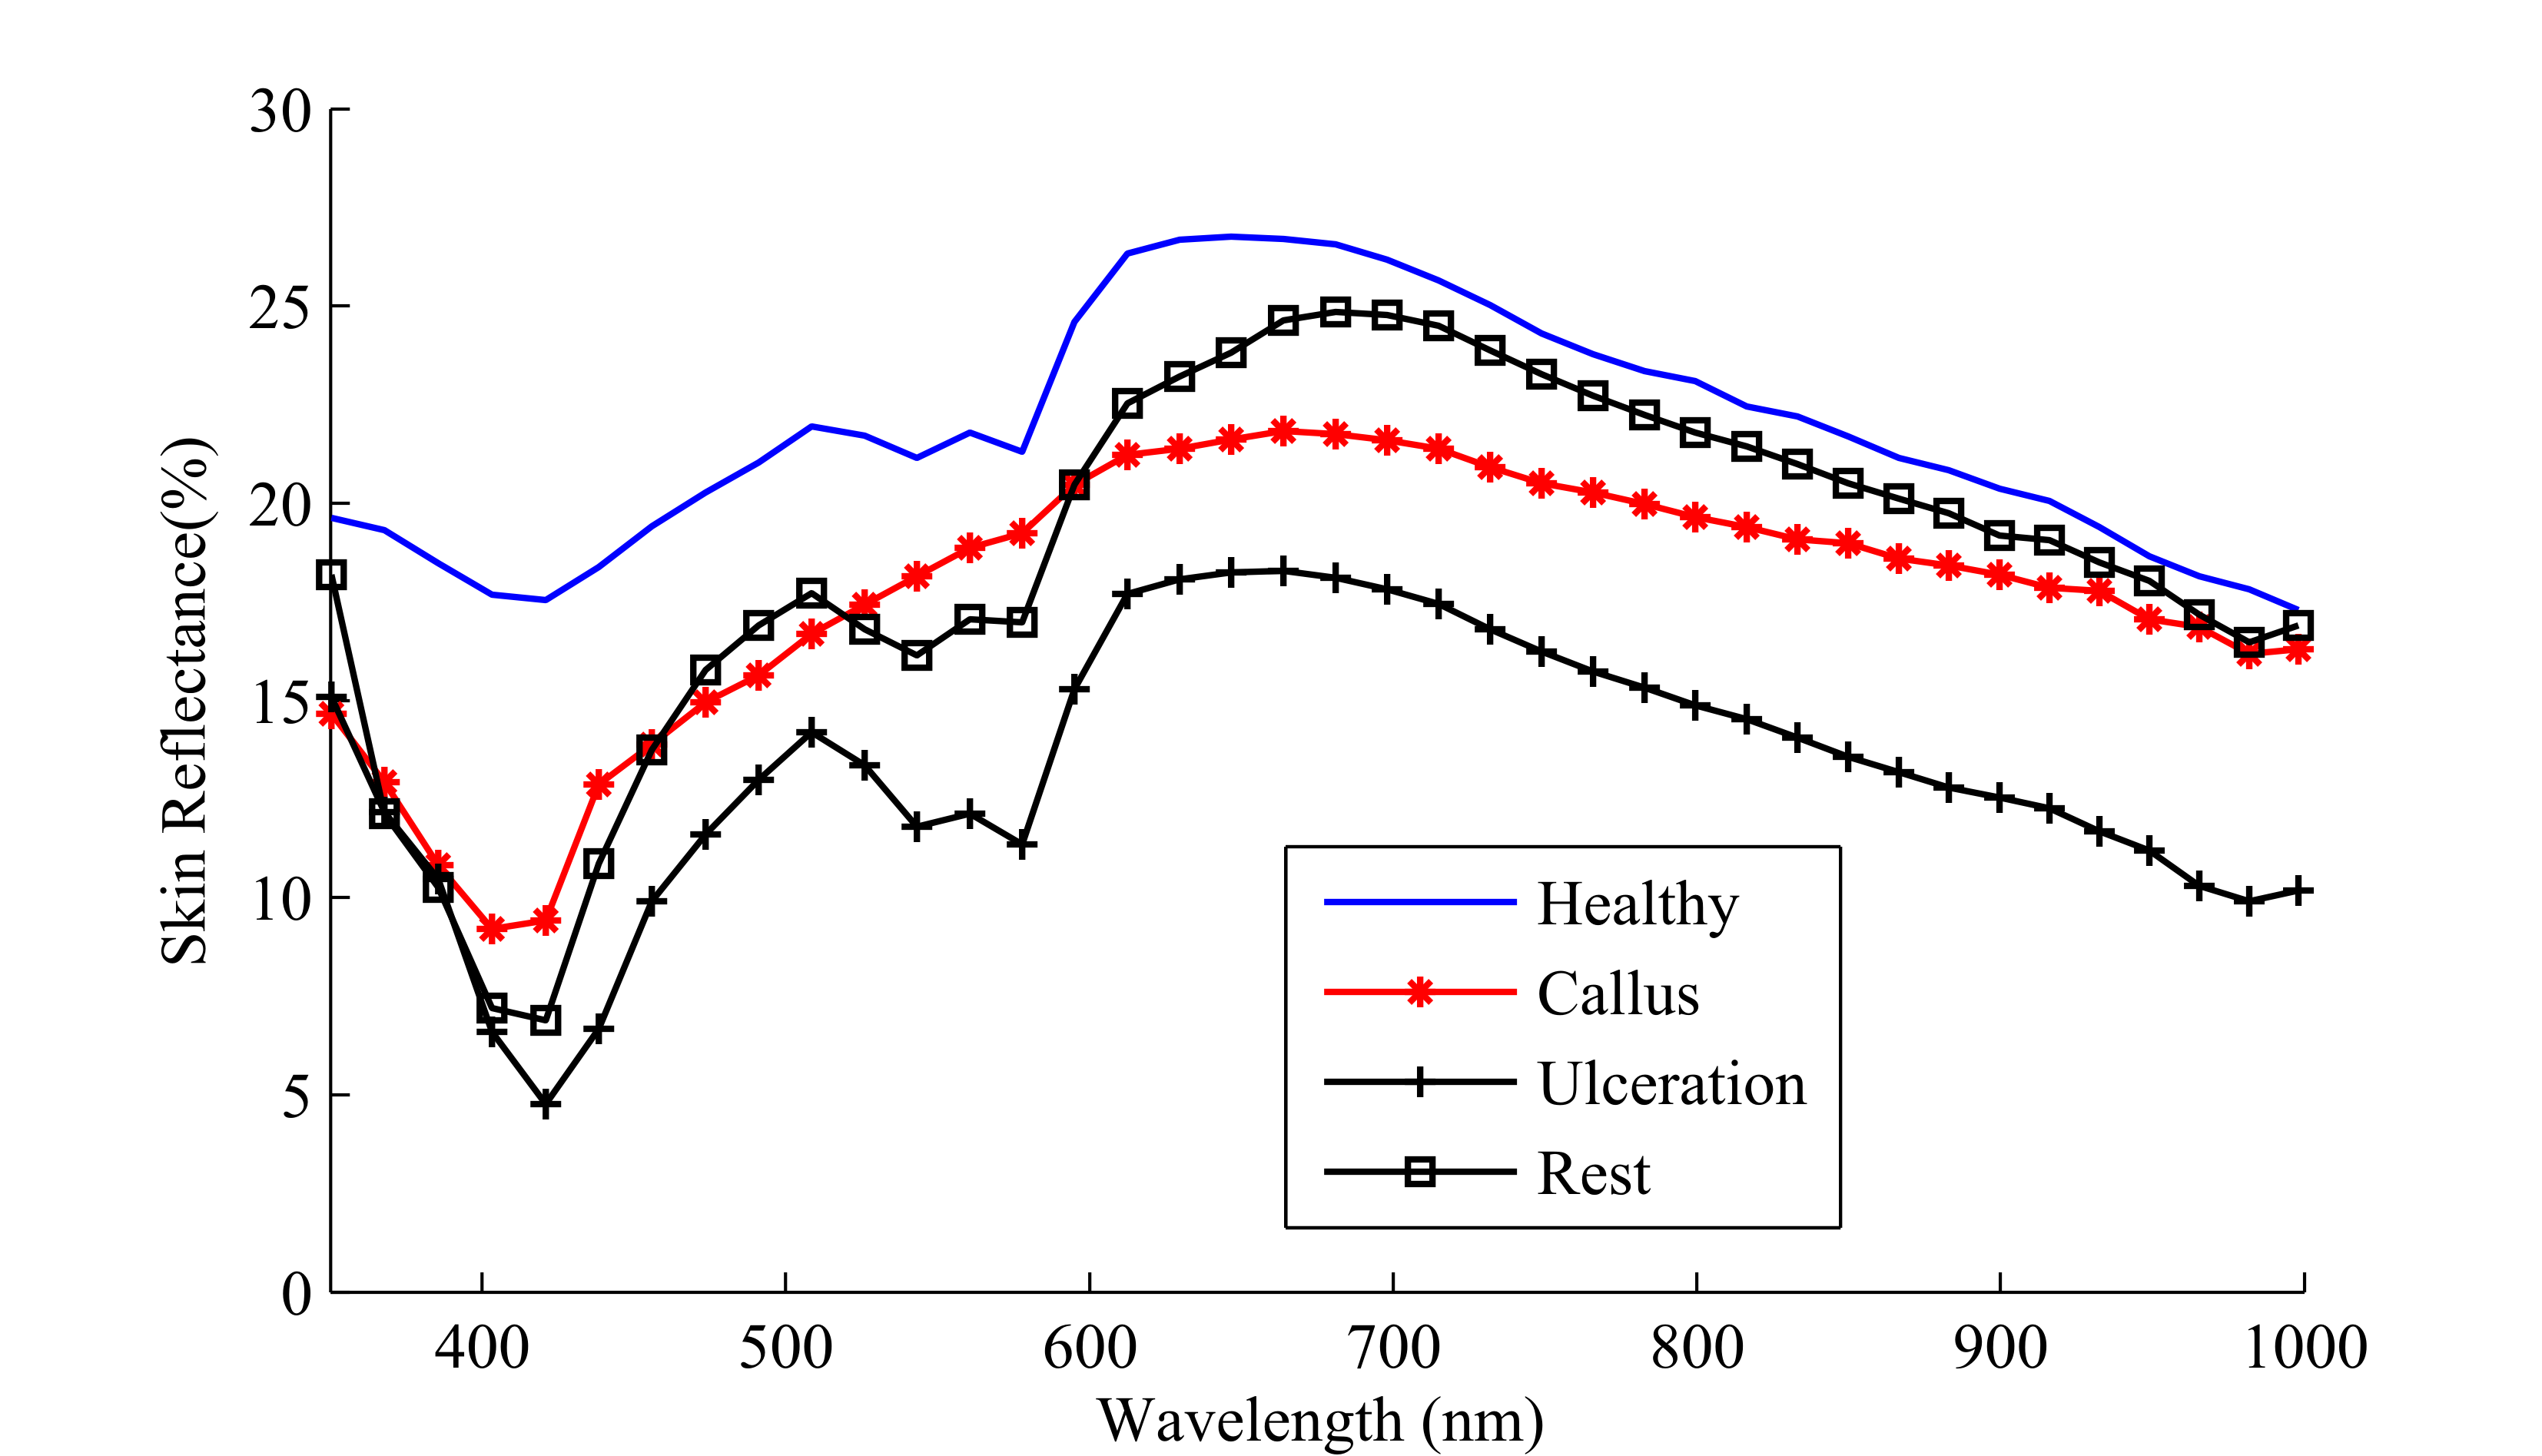
\includegraphics[width=2.5in, height=1.4in]{examples.png}
        \caption{Examples of spectrum from different classes}
        \label{fig:example}
\end{figure}

% Note that IEEE typically puts floats only at the top, even when this
% results in a large percentage of a column being occupied by floats.


% An example of a double column floating figure using two subfigures.
% (The subfig.sty package must be loaded for this to work.)
% The subfigure \label commands are set within each subfloat command, the
% \label for the overall figure must come after \caption.
% \hfil must be used as a separator to get equal spacing.
% The subfigure.sty package works much the same way, except \subfigure is
% used instead of \subfloat.
%
%\begin{figure*}[!t]
%\centerline{\subfloat[Case I]\includegraphics[width=2.5in]{subfigcase1}%
%\label{fig_first_case}}
%\hfil
%\subfloat[Case II]{\includegraphics[width=2.5in]{subfigcase2}%
%\label{fig_second_case}}}
%\caption{Simulation results}
%\label{fig_sim}
%\end{figure*}
%
% Note that often IEEE papers with subfigures do not employ subfigure
% captions (using the optional argument to \subfloat), but instead will
% reference/describe all of them (a), (b), etc., within the main caption.


% An example of a floating table. Note that, for IEEE style tables, the 
% \caption command should come BEFORE the table. Table text will default to
% \footnotesize as IEEE normally uses this smaller font for tables.
% The \label must come after \caption as always.
%
\begin{table}[!t]
%% increase table row spacing, adjust to taste
\renewcommand{\arraystretch}{1.3}
% if using array.sty, it might be a good idea to tweak the value of
%\extrarowheight as needed to properly center the text within the cells
\caption{An Example of a Table}
\label{table_example}
\centering
%% Some packages, such as MDW tools, offer better commands for making tables
%% than the plain LaTeX2e tabular which is used here.
\begin{tabular}{|c||c|}
\hline
One & Two\\
\hline
Three & Four\\
\hline
\end{tabular}\label{tab:example}
\end{table}


% Note that IEEE does not put floats in the very first column - or typically
% anywhere on the first page for that matter. Also, in-text middle ("here")
% positioning is not used. Most IEEE journals use top floats exclusively.
% Note that, LaTeX2e, unlike IEEE journals, places footnotes above bottom
% floats. This can be corrected via the \fnbelowfloat command of the
% stfloats package.









% if have a single appendix:
%\appendix[Proof of the Zonklar Equations]
% or
%\appendix  % for no appendix heading
% do not use \section anymore after \appendix, only \section*
% is possibly needed

% use appendices with more than one appendix
% then use \section to start each appendix
% you must declare a \section before using any
% \subsection or using \label (\appendices by itself
% starts a section numbered zero.)
%



\section{Matlab scripts}


\lstset{language=Matlab,%
basicstyle=\tiny\ttfamily,
breaklines=true,%
morekeywords={matlab2tikz},
keywordstyle=\color{NavyBlue},%
morekeywords=[2]{1}, keywordstyle=[2]{\color{black}},
identifierstyle=\color{black},%
stringstyle=\color{OrangeRed},
commentstyle=\color{OliveGreen},%
showstringspaces=false,%without this there will be a symbol in the places where there is a space
numbers=left,%
numberstyle={\tiny\color{gray}\scalebox{.8}},% size of the numbers
numbersep=3pt, % this defines how far the numbers are from the text
%emph=[1]{for,end,break},emphstyle=[1]\color{red}, %some words to emphasise
%emph=[2]{word1,word2}, emphstyle=[2]{style}, 
}

%\lstinputlisting{convertvideo.m}
\subsection{main}
\label{sec:main}
\lstinputlisting[language=Matlab]{../main.m}

\subsection{removeBackground}
\label{sec:removeBackground}
\lstinputlisting[language=Matlab]{../removeBackground.m}

\subsection{normalizeImages}
\label{sec:normalizeImages}
\lstinputlisting[language=Matlab]{../normalizeImages.m}

\subsection{mapDisparity}
\label{sec:mapDisparity}
\lstinputlisting[language=Matlab]{../mapDisparity.m}

\subsection{relaxgaps}
\label{sec:relaxgaps}
\lstinputlisting[language=Matlab]{../relaxgaps.m}

\subsection{laplacianFilter}
\label{sec:laplacianFilter}
\lstinputlisting[language=Matlab]{../laplacianFilter.m}

\subsection{facemesh}
\label{sec:facemesh}
\lstinputlisting[language=Matlab]{../facemesh.m}



% you can choose not to have a title for an appendix
% if you want by leaving the argument blank
\section{Guideline for References}
In text, refer simply to the reference number. Do not use �Ref.� or �reference� except at the beginning of a sentence: �Reference [3] shows ... .� 




% Can use something like this to put references on a page
% by themselves when using endfloat and the captionsoff option.
\ifCLASSOPTIONcaptionsoff
  \newpage
\fi



% trigger a \newpage just before the given reference
% number - used to balance the columns on the last page
% adjust value as needed - may need to be readjusted if
% the document is modified later
%\IEEEtriggeratref{8}
% The "triggered" command can be changed if desired:
%\IEEEtriggercmd{\enlargethispage{-5in}}

% references section

% can use a bibliography generated by BibTeX as a .bbl file
% BibTeX documentation can be easily obtained at:
% http://www.ctan.org/tex-archive/biblio/bibtex/contrib/doc/
% The IEEEtran BibTeX style support page is at:
% http://www.michaelshell.org/tex/ieeetran/bibtex/
%\bibliographystyle{IEEEtran}
% argument is your BibTeX string definitions and bibliography database(s)
%\bibliography{IEEEabrv,../bib/paper}
%
% <OR> manually copy in the resultant .bbl file
% set second argument of \begin to the number of references
% (used to reserve space for the reference number labels box)
\begin{thebibliography}{1}

\bibitem{IEEEhowto:kopka}
H.~Kopka and P.~W. Daly, \emph{A Guide to \LaTeX}, 3rd~ed.\hskip 1em plus
  0.5em minus 0.4em\relax Harlow, England: Addison-Wesley, 1999.

\end{thebibliography}

% biography section
% 
% If you have an EPS/PDF photo (graphicx package needed) extra braces are
% needed around the contents of the optional argument to biography to prevent
% the LaTeX parser from getting confused when it sees the complicated
% \includegraphics command within an optional argument. (You could create
% your own custom macro containing the \includegraphics command to make things
% simpler here.)
%\begin{biography}[{\includegraphics[width=1in,height=1.25in,clip,keepaspectratio]{mshell}}]{Michael Shell}
% or if you just want to reserve a space for a photo:

%\begin{IEEEbiography}{Michael Shell}
%Biography text here.
%\end{IEEEbiography}

% if you will not have a photo at all:
%\begin{IEEEbiographynophoto}{John Doe}
%Biography text here.
%\end{IEEEbiographynophoto}

% insert where needed to balance the two columns on the last page with
% biographies
%\newpage

%\begin{IEEEbiographynophoto}{Jane Doe}
%Biography text here.
%\end{IEEEbiographynophoto}

% You can push biographies down or up by placing
% a \vfill before or after them. The appropriate
% use of \vfill depends on what kind of text is
% on the last page and whether or not the columns
% are being equalized.

%\vfill

% Can be used to pull up biographies so that the bottom of the last one
% is flush with the other column.
%\enlargethispage{-5in}



% that's all folks
\end{document}


